\chapter{Implementation}
\label{chapter:Implementation}
This chapter summarizes the implementation for crucial parts of the recovery system implemented for this thesis.
§\ref{section:RecoveringFragmentsAnParthoodLinks} covers the implementation of \gls{Fragment} and \gls{Parthood} link recovery.
§\ref{section:RecoveringCorrespondenceAndConformanceLinks} covers the implementation of \gls{Correspondence} and \gls{Conformance} link recovery

\section{Recovering Fragments \& Parthood Links}
\label{section:RecoveringFragmentsAnParthoodLinks}
This section summarizes the implementation of \gls{Fragment} recovery.
\Glspl{Fragment} are syntactically well-formed pieces of code.
For instance, consider the \gls{Java} class in listing \ref{listing:ExcerptOfTheCompanyJavaClass}.
\begin{lstlisting}[language=Java,caption={Excerpt of the Company Java class},label={listing:ExcerptOfTheCompanyJavaClass}]
public class Company {
	...
	private String name;
	...
	public String getName() {
		return name;
	}
	...
}
\end{lstlisting}
It consists, among others, of the following fragments:
\begin{itemize}
\item
a field declaration fragment for \texttt{name}:
\begin{lstlisting}[language=Java,numbers=none,frame=no]
private String name;
\end{lstlisting}
\item
a method declaration fragment for an accessor-method of \texttt{name}:
\begin{lstlisting}[language=Java,numbers=none,frame=no]
public String getName() {
	return name;
}
\end{lstlisting}
\item
the return statement of the accessor-method:
\begin{lstlisting}[language=Java,numbers=none,frame=no]
return name;
\end{lstlisting}
\item
the class declaration itself can also be considered a fragment.
\end{itemize}

The task of recovering \glspl{Fragment} is to add entities for each of such code pieces into a megamodel.
Figure \ref{figure:IdealizedRecoveryOfJavaFragments} exemplifies the recovery of \gls{Java}\footnote{Recovery for \gls{XML} and \gls{SQL/DDL} is implemented in a similar fashion.
If there is a noteworthy difference for other languages it will be explored, otherwise we keep using \gls{Java} as example domain for the remaining sections of §\ref{section:RecoveringFragments}.} \glspl{Fragment} in an idealized form:
\begin{figure}[h!]
\begin{center}
\begin{minipage}{0.5\textwidth}
\begin{lstlisting}[language=Java,numbers=none]
public class Company {
	...
	private String name;
	...
	public String getName() {
		return name;
	}
	...
}
\end{lstlisting}
\end{minipage}
\\\vspace*{5mm}
{
\LARGE
\bfseries
$\downarrow$
}
\\\vspace*{5mm}
\resizebox{\textwidth}{!}{
\Tree [.Class \texttt{public} \texttt{class}
	[.ID \texttt{Company} ]
	\texttt{$\lbrace$}
	[.Members 
		[.Member \texttt{...} ]
		[.Member \texttt{public} [.Type \texttt{String} ] [.ID \texttt{name} ] \texttt{;} ]
		[.Member \texttt{...} ]
		[.Member \texttt{public} [.Type \texttt{String} ] [.ID \texttt{getName} ] \texttt{(} \texttt{)}
		\texttt{$\lbrace$}
		[.Statements
			[.Statement \texttt{return} \texttt{name} \texttt{;} ]
		]
		\texttt{$\rbrace$}
		]
		[.Member \texttt{...} ]
	]
	\texttt{$\rbrace$}
]
}
\\\vspace*{5mm}
{
\LARGE
\bfseries
$\downarrow$
}
\\\vspace*{5mm}
\resizebox{\textwidth}{!}{
\Tree [.Class
[.\texttt{public class Company \{ private String name; public String getName() \{ return name; \} \}}
	[.Fields 
		[.Field \texttt{...} ] 
		[.Field \texttt{private String name;} ] 
		[.Field \texttt{...} ] 
	]
	[.Methods 
		[.Method \texttt{...} ]
		[.Method \texttt{public String getName() \{ return name; \}} ]
		[.Method \texttt{...} ]
	]
]]
}
\\\vspace*{5mm}
{
\LARGE
\bfseries
$\downarrow$
}
\\\vspace*{5mm}
\begin{minipage}{0.5\textwidth}
\begin{lstlisting}[numbers=none]
Company : Fragment
Company elementOf JavaClassFragments
Company fragmentOf artifact
...
Company.name : Fragment
Company.name elementOf JavaFieldFragments
Company.name fragmentOf Company
...
Company.getName : Fragment
Company.getName elementOf JavaMethodFragments
Company.getName fragmentOf Company
\end{lstlisting}
\end{minipage}
\end{center}
{
\scriptsize
This picture shows an idealized recovery of \gls{Java} \glspl{Fragment}:
\begin{center}
code \gls{Artifact}
$\rightarrow$
\gls{ParseTree}
$\rightarrow$
\gls{Fragment} \gls{AST}
$\rightarrow$
\gls{Megamodel}
\end{center} 
Both \gls{ParseTree} and \gls{AST} are depicted in a simplified, schematic form.
}
\caption{Idealized Recovery of Java Fragments}
\label{figure:IdealizedRecoveryOfJavaFragments}
\end{figure}
\begin{enumerate}
\item
a \gls{ParseTree} is generated from an artifact; this is done via \gls{ANTLR} as described in §\ref{subsubsection:SyntaxAnalysisAPI} and does not require further explanation, since it is only an application of the most common \gls{ANTLR} use case
\item
then the \gls{ParseTree} is transformed into an concrete \gls{Fragment} \gls{AST} model; this is also done relying on \gls{ANTLR} tree traversal utilities and described in detail in §\ref{subsection:ConcreteFragmentModels}
\item
eventually, nodes of the generated \gls{Fragment} \gls{AST} are added to a \gls{Megamodel} as entities; the details are described in §\ref{subsection:MegamodelingFragments}.
\end{enumerate}



\subsection{Concrete Fragment Models}
\label{subsection:ConcreteFragmentModels}
As mentioned in §\ref{subsubsection:AbstractFragmentModel}, Concrete \Gls{Fragment} Models are derivations of the Abstract Fragment Model of the Recovery System \gls{API}.
Figure \ref{figure:JavaFragmentASTModel} shows an \gls{UML} class diagram of the implemented \Gls{Fragment} \gls{AST} for \gls{Java}.
\begin{figure}[h!]
\begin{center}
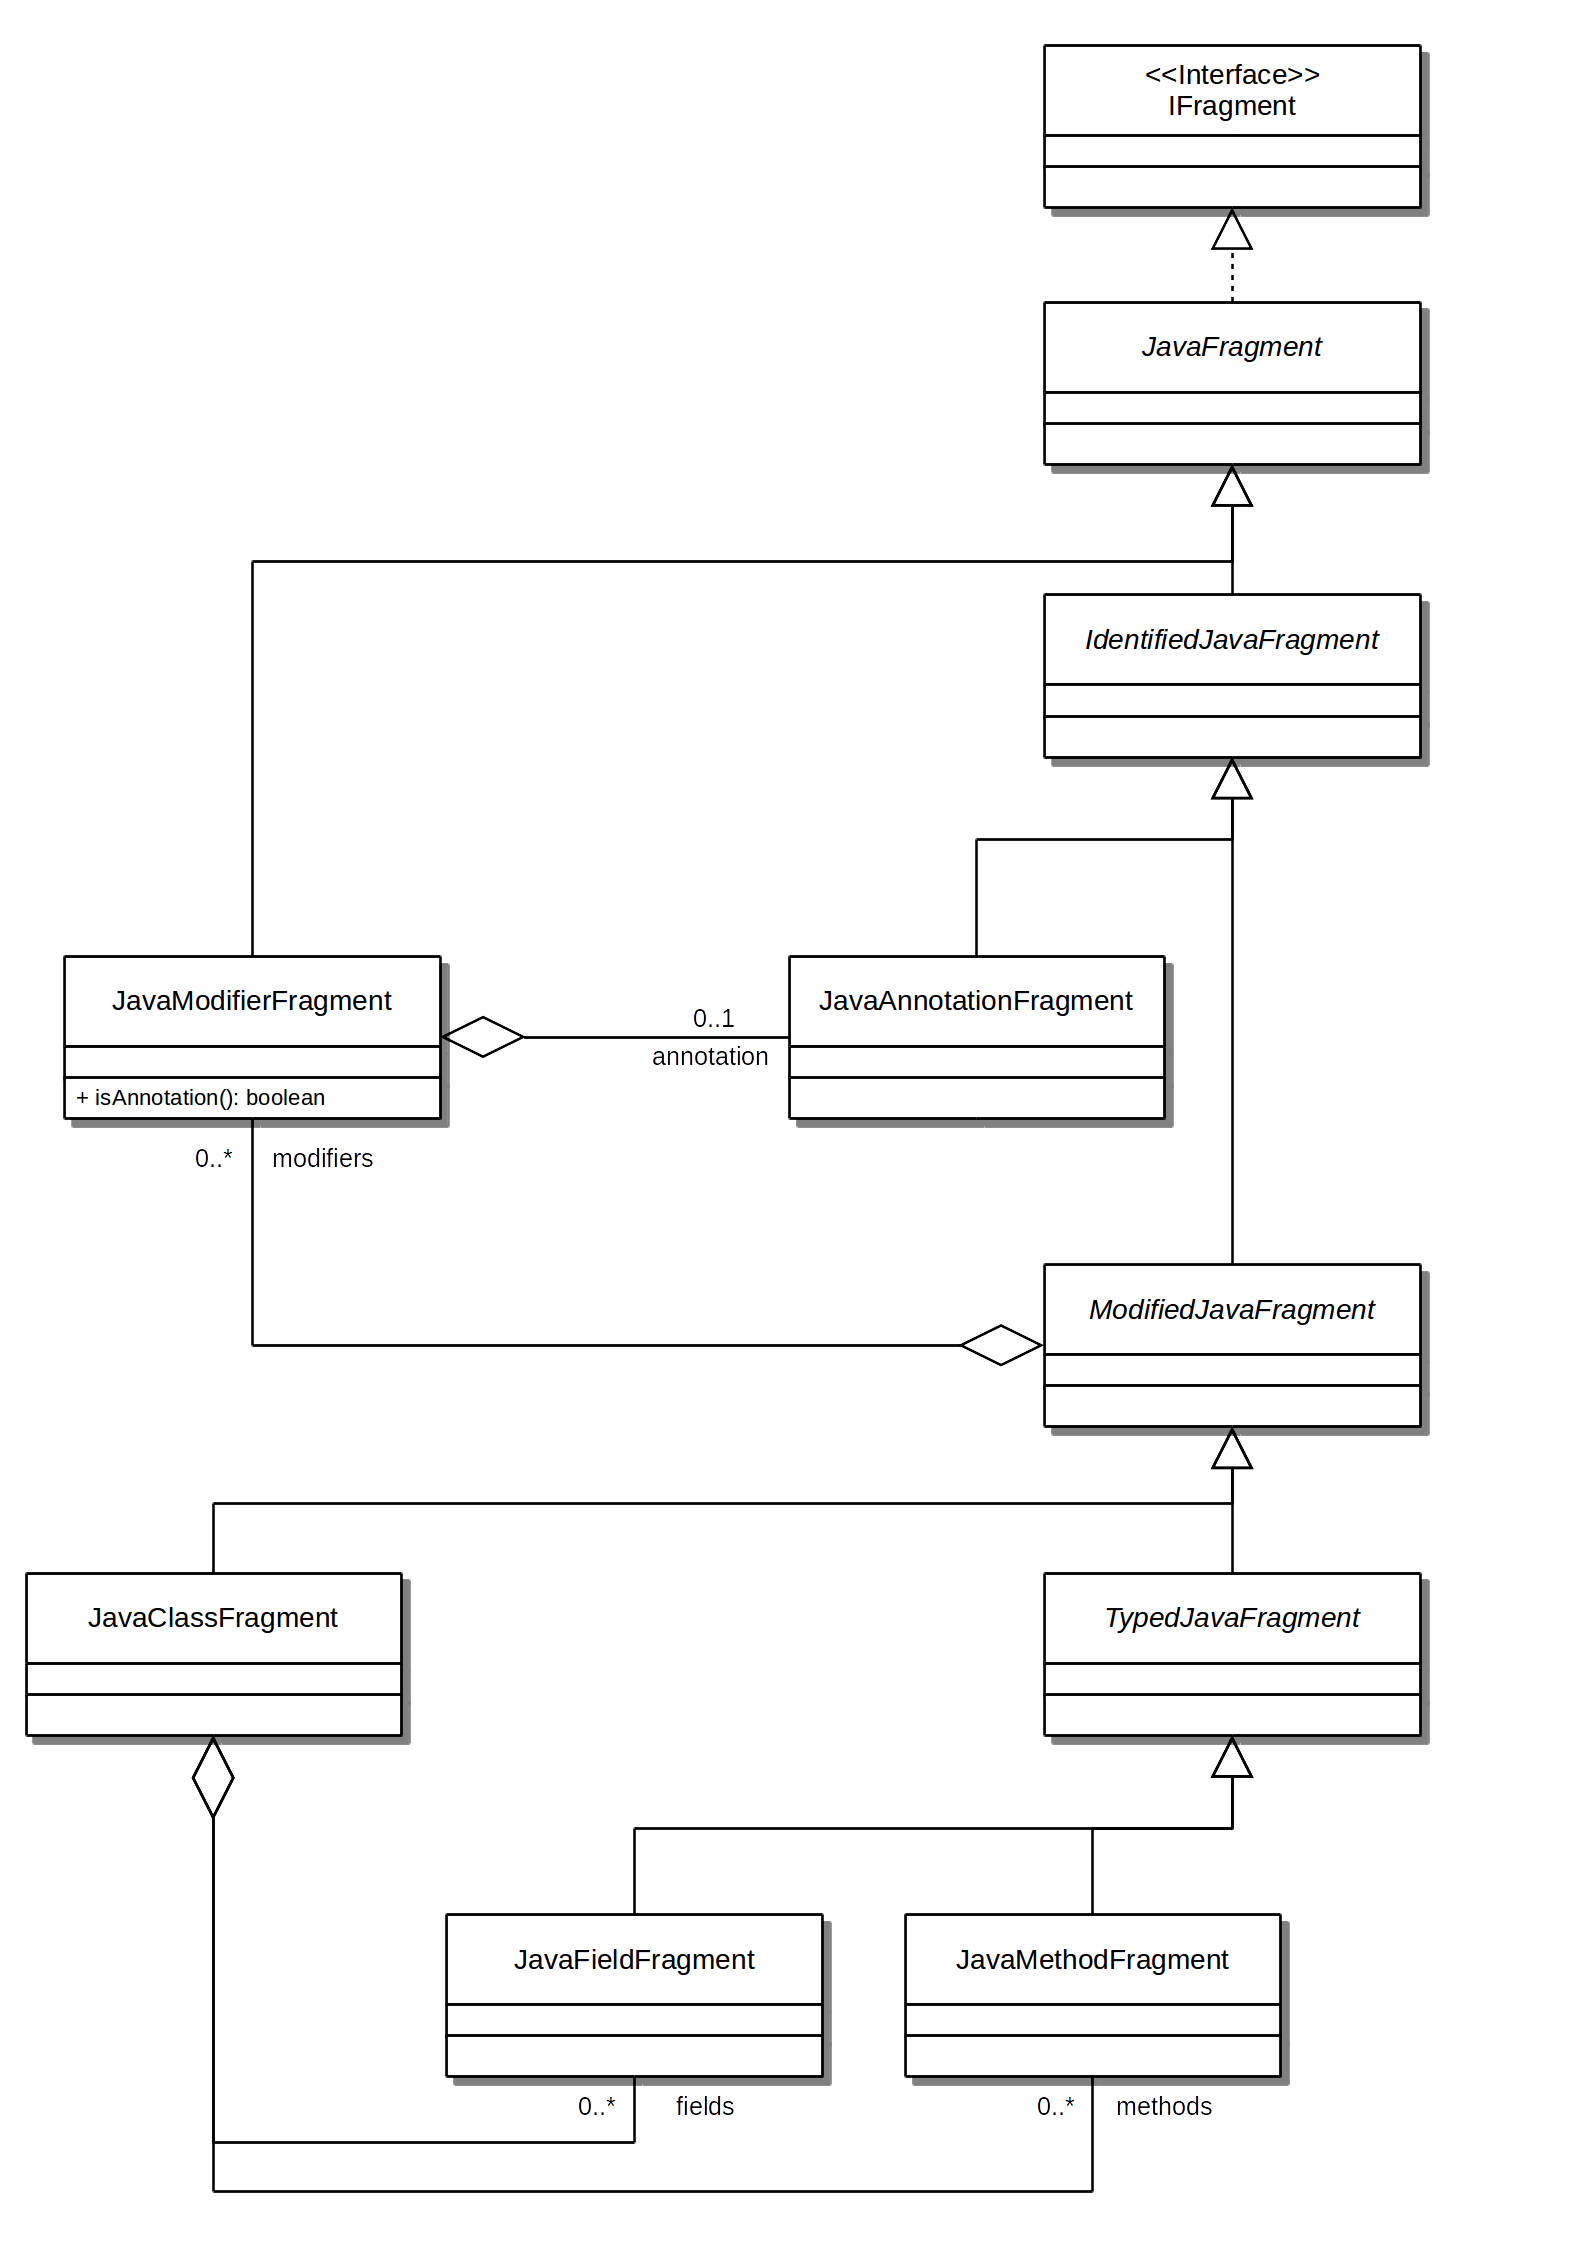
\includegraphics[width=.7\textwidth]{images/JavaFragmentModel.png}
\end{center}
\caption{Java Fragment AST Model}
\label{figure:JavaFragmentASTModel}
\end{figure}
All \gls{Fragment} classes derive from \texttt{IFragment} through the base class \texttt{JavaFragment}.
From here, several specializations are introduced:
\begin{itemize}
\item
\texttt{IdentfiedJavaFragment} for constructs with identifiers
\item
\texttt{ModifiedJavaFragment} for constructs with modifiers like \texttt{private, public, final, abstract, static}, etc. or annotation meta-data
\item
\texttt{TypedJavaFragment} for constructs with a distinct (return-) type like fields, methods or variables
\end{itemize}
The \gls{Fragment} model for \gls{Java} only focuses on structural syntactical features of the language.
Everything below method signature level is omitted, because \glspl{Fragment} of this level are not important for the scope of this thesis.
On the other hand, annotations are captured, since they provide significant information for further recovery analysis.
\gls{Hibernate} and \gls{JAXB} rely on annotations for \gls{O/R/X-Mapping}.

The \gls{AST} is constructed using the \gls{ANTLR} \texttt{ParseTreeListener} approach as described in §\ref{subsubsection:SyntaxAnalysisAPI}.
\begin{lstlisting}[language=Java,caption={Construction of Java Fragment ASTs},label={listing:JavaFragmentASTConstruction}]
...
@Override
public void exitMethodDeclaration(Java8Parser.MethodDeclarationContext ctx) {
    javaMethodFragments.push(java8FragmentFactory.newJavaMethodFragment(ctx, javaMethodModifierFragments));
}

@Override
public void exitNormalClassDeclaration(Java8Parser.NormalClassDeclarationContext ctx) {
    javaClassFragments.push(java8FragmentFactory.newJavaClassFragment(ctx, javaClassModifierFragments, javaFieldFragments, javaMethodFragments, declaredPackage));
}
...
\end{lstlisting}
Listing \ref{listing:JavaFragmentASTConstruction} shows an excerpt from the listener implementation used to construct the the \gls{AST} for \gls{Java} \glspl{Fragment}.
%This snippet in listing \ref{listing:JavaFragmentASTConstruction} shows an excerpt of the listener used to construct \gls{Java} \gls{Fragment} \glspl{AST}.
Here, fragment instances are created when the listener leaves certain nodes of the \gls{ParseTree}.
Creation is delegated to a factory.
The listener pushes fragments onto stacks, making the overall implementation work like a pushdown automaton or stack machine.



\subsection{Megamodeling Fragments}
\label{subsection:MegamodelingFragments}
In order to add \glspl{Fragment} into a \gls{Megamodel}, a suitable linguistic model has to be declared first. 
Consider the following instance level \gls{Megamodel} of recovered \glspl{Fragment} shown in listing \ref{listing:AMegamodelForFragmentsOfAJavaClass}.
\begin{lstlisting}[caption={A Megamodel for fragments of a Java class},label={listing:AMegamodelForFragmentsOfAJavaClass}]
File < Artifact
Fragment < Artifact
...
elementOf < Set * Set
fragmentOf < Fragment * Artifact
...
aJavaFile : File
aJavaFile = 'Company.java'
...
aJavaFile.Company : Fragment
aJavaFile.Company elementOf JavaClassFragments
aJavaFile.Company fragmentOf aJavaFile
...
aJavaFile.Company.name : Fragment
aJavaFile.Company.name elementOf JavaFieldFragments
aJavaFile.Company.name fragmentOf aJavaFile
aJavaFile.Company.name fragmentOf Company
...
aJavaFile.Company.getName : Fragment
aJavaFile.Company.getName elementOf JavaMethodFragments
aJavaFile.Company.getName fragmentOf aJavaFile
aJavaFile.Company.getName fragmentOf Company
\end{lstlisting}
This \gls{Megamodel} shows \glspl{Fragment} of a \gls{Java} file \texttt{Company.java}.
It contains entities denoting a class declaration, a field declaration and a method declaration \gls{Fragment}.
All are declared instances of the entity type \texttt{Fragment}.
Entity names use dot-notation for implying \gls{Parthood}, i.e.:
\begin{align*}
a.b \Rightarrow b ~ \partOf ~ a
\end{align*}
Further details of the naming-scheme employed for \gls{Fragment} entities are explored in §\ref{subsubsection:FragmentEntityIdentifiers}.

We use \texttt{elementOf} for further specialization and/or generalization of the entitie's kind\footnote{We use the term \textit{kind} to avoid confusion with entity types, although we use it to refer to \gls{Fragment} types.}.
However, the right-hand side of these relationships used to specialize \glspl{Fragment} are not simply sets, they are actually modeled as languages as we will see in §\ref{subsubsection:FragmentLanguages}.

\subsubsection{Fragment Languages}
\label{subsubsection:FragmentLanguages}
A \gls{Fragment} alone cannot be element of the language the artifact it originated from belongs to, e.g. \gls{Java} methods alone cannot be accepted by the \gls{Java} grammar, nor can \gls{XML} attributes alone be accepted by the \gls{XML} grammar.
Therefore, in order to cleanly add \glspl{Fragment} into a \gls{Megamodel}, we need to model \gls{Fragment} languages.
Listing \ref{listing:JavaFragmentMegamodel} shows the \gls{Megamodel} for \gls{Java} \glspl{Fragment}.
\begin{lstlisting}[caption={A Megamodel for Java Fragment},label={listing:JavaFragmentMegamodel}]
...
Language < Set
...
fragmentLanguageOf < Language * Language
...
Java : Language

JavaFragments : Language
JavaFragments fragmentLanguageOf Java

JavaClassFragments : Language
JavaClassFragments subsetOf JavaFragments

JavaFieldFragments : Language
JavaFieldFragments subsetOf JavaFragments

JavaMethodFragments : Language
JavaMethodFragments subsetOf JavaFragments
...
\end{lstlisting}
It introduces the special relationship type \texttt{fragmentLanguageOf}, denoting the left-hand side is the language containing all possible \glspl{Fragment}  the right-hand side's language elements can be deconstructed in.
This also implies a super-set relation between the two languages as \fragmentOf~ is reflexive like \partOf, so:
\begin{align*}
L_1 \texttt{~fragmentLanguageOf~} L_2 \Rightarrow L_2 \subseteq L_1
\end{align*}

\subsubsection{Fragment Entity Identifiers}
\label{subsubsection:FragmentEntityIdentifiers}
\gls{MegaL} entity identifiers have to be unique, but names of the constructs represented by \gls{Fragment} do not necessarily adhere to that.
For instance, a \gls{Java} method may be overloaded or multiple \gls{XML} elements are naturally identified via the same name.
Because of this, a naming scheme for storing recovered \glspl{Fragment} in a \gls{MegaL} \gls{Megamodel} needs to be devised.

We utilize a simple naming scheme, preserving both uniqueness and readability.
Consider listing \ref{listing:ExcerptOfACompanyXMLFile}, showing an excerpt of a \gls{XML} file.
\begin{lstlisting}[caption={Excerpt of a Company XML file},label={listing:ExcerptOfACompanyXMLFile}]
<company id="0" name="Softlang Inc.">
    <departments>
        <department id="0" name="Grammar Engineering">
			...
        </department>
        <department id="1" name="Research &amp; Development">
            ...
        </department>
        ...
    </departments>
</company>
\end{lstlisting}
If we want to add both \texttt{department} \glspl{Fragment} to a \gls{Megamodel}, we prepend an indexing prefix to its name, i.e. \texttt{F<index>\$}.
This is exemplified in listing \ref{listing:QualifiedFragmentIdentifiers}.
\begin{lstlisting}[caption={Qualified Fragment Identifiers},label={listing:QualifiedFragmentIdentifiers}]
xmlFile : File
xmlFile.company : Fragment
xmlFile.company.departments : Fragment
xmlFile.company.departments.F0$department : Fragment
xmlFile.company.departments.F1$department : Fragment
\end{lstlisting}


\subsection{Recovering Parthood Links}
\label{subsection:RecoveringParthoodLinks}
This section summarizes the implementation of \gls{Parthood} link recovery.
Recovering \gls{Parthood} links exploits the nature of \glspl{ParseTree} and \glspl{AST} as mentioned §\ref{subsubsection:MereologicalFragmentAnalysisAPI}, where the nested structure of code is represented by parent/child association between nodes.
Listing \ref{listing:PseudoCodeRecoveryOfParthoodLinks} shows recovery of \gls{Parthood} links from a tree data structure in pseudo code notation.
\begin{lstlisting}[caption={Pseudo code Recovery of Parthood Links},label={listing:PseudoCodeRecoveryOfParthoodLinks},morekeywords={procedure,foreach,input,output}]
input: A node n of a n-ary tree structure.
procedure recoverParthoodLinks(n):
	foreach child node c of n:
		declare c partOf n.
		recoverParthoodLinks(c).	
\end{lstlisting}
The recovery procedure utilizes recursive descent traversal on a tree.
The actual implementation of \gls{Parthood} link recovery adds \partOf- and \fragmentOf-links simultaneously into a simple knowledge base backed by a graph data structure.
Listing \ref{listing:ActualRecoveryOfParthoodLinks} shows the responsible methods for this.
\begin{lstlisting}[language=Java,caption={Actual Recovery of Parthood Links},label={listing:ActualRecoveryOfParthoodLinks}]
private IFragmentKBBuilder newFragmentKB(IFragmentKBBuilder fragmentKBBuilder, IFragment fragment) {
    for (IFragment child : fragment.getChildren()) {
        fragmentKBBuilder = newFragmentKB(fragmentKBBuilder.fragmentOf(child, fragment), child);
    }
    return fragmentKBBuilder;
}

@Override
public IFragmentKB newFragmentKB(IFragment fragment) {
	return newFragmentKB(fragmentKBBuilderFactory.newFragmentKBBuilder(), fragment).build();
}
\end{lstlisting}

Once a graph of recovered \partOf- and/or \fragmentOf-links is present, we can compute its transitive closure, thus recovering transitive \partOf- and \fragmentOf-links.
Listing \ref{listing:PseudoCodeRecoveryOfTramsotoveParthoodLinks} shows the pseudo code for computing the transitive closure of a graph.
\begin{lstlisting}[caption={Pseudo code Recovery of transitive Parthood Links},label={listing:PseudoCodeRecoveryOfTramsotoveParthoodLinks},morekeywords={procedure,foreach,input,output,if,yield}]
input: A graph g and vertex v.
procedure reachableVertices(g,v):
	mark v as walked.
	foreach adjacent vertex w of v:
		if w is not marked as walked:
			yield w.
			reachableVertices(g,w).
			
input: A graph g.
procedure computeTransitiveClosure(g):
	foreach vertex v of g:
		foreach vertex w in reachableVertices(g,v):
			if w != v and g does neither contain edge (v,w) nor (w,v):
				add edge (v,w) to g.
\end{lstlisting}
Note, the pseudo code implementation for computation of transitive closures uses a recursive \gls{DFS} for computing transitively reachable vertices of a given vertex.
It utilizes a yield-return, denoting the next value is available from the outside without exiting the procedure.
This can be thought of sequence which would be returned normally.
The actual implementation utilizes the \gls{IteratorPattern} and non-recursive \gls{DFS} for computing transitively reachable vertices. 

\section{Recovering Correspondence \& Conformance Links}
\label{section:RecoveringCorrespondenceAndConformanceLinks}
This section summarizes the implementation of \gls{Correspondence} and \gls{Conformance} link recovery.
Recovering  \gls{Correspondence} and \gls{Conformance} links is done by implementing heuristics for the Comparative Fragment Analysis \gls{API}, as mentioned in §\ref{subsubsection:ComparativeFragmentAnalysisAPI}.
Heuristics are strategies in sense of the \gls{StrategyPattern}.
They are used for traversing two \glspl{AST} and comparing nodes in a non-probabilistic yet not absolutely correct deterministic way.
They employ simple string comparison methods like plural removal, that is deletion of the English plural, and letter case normalization for detecting similarities.
This heavily relies on conventions implemented in technologies, e.g. \gls{JAXB}, where \gls{Java} field identifiers are used as \gls{XML} element names, if not declared otherwise.
In case, a \gls{Java} annotation provides an explicit name, it is used with strict equivalence.

Listings \ref{listing:ExcerptOfTheBaseXmlXsdSimilarityHeuristicClass} and \ref{listing:TheXmlXsdSimilarityHeuristicClass} shows excerpts of the heuristics implemented to uncover related elements among \gls{XML} and \gls{XSD} \glspl{Fragment}.
It uses an abstract base class (listing \ref{listing:ExcerptOfTheBaseXmlXsdSimilarityHeuristicClass}) for traversing \gls{Fragment} \glspl{AST} and a concrete class for specifying comparison predicates (listing \ref{listing:TheXmlXsdSimilarityHeuristicClass}).
\begin{lstlisting}[language=Java,caption={Excerpt of the BaseXmlXsdSimilarityHeuristic class},label={listing:ExcerptOfTheBaseXmlXsdSimilarityHeuristicClass}]
public abstract class BaseXmlXsdSimilarityHeuristic implements IFragmentAnalyzerHeuristic {

    protected abstract boolean areSimilar(XmlElementFragment xmlElementFragment, XmlElementFragment xsdElementFragment);
    protected abstract boolean areSimilar(XmlAttributeFragment xmlAttributeFragment, XmlElementFragment xsdElementFragment);

    ...

    private void addSimilarities(IBinaryRelation<IFragment> similarities, XmlElementFragment xmlElementFragment, XmlElementFragment xsdElementFragment) {
        if (areSimilar(xmlElementFragment, xsdElementFragment)) {
            similarities.add(xmlElementFragment, xsdElementFragment);
            for (XmlAttributeFragment xmlAttributeFragment : xmlElementFragment.getXmlAttributeFragments()) {
                addSimilarities(similarities, xmlAttributeFragment, xsdElementFragment.getXmlElementFragments());
            }
        }
        for(XmlElementFragment xsdElementFragment1 : xsdElementFragment.getXmlElementFragments()) {
            addSimilarities(similarities, xmlElementFragment, xsdElementFragment1);
        }
        for(XmlElementFragment xmlElementFragment1 : xmlElementFragment.getXmlElementFragments()) {
            addSimilarities(similarities, xmlElementFragment1, xsdElementFragment);
        }
        addSimilarities(similarities, xmlElementFragment.getXmlElementFragments(), xsdElementFragment.getXmlElementFragments());
    }

    ...
}
\end{lstlisting}

\begin{lstlisting}[language=Java,caption={The XmlXsdSimilarityHeuristic class},label={listing:TheXmlXsdSimilarityHeuristicClass}]
public class XmlXsdSimilarityHeuristic extends BaseXmlXsdSimilarityHeuristic {
    @Override
    protected boolean areSimilar(XmlElementFragment xmlElementFragment, XmlElementFragment xsdElementFragment) {
        return (XmlFragmentUtils.isXsElementTag(xsdElementFragment)
                || XmlFragmentUtils.isXsComplexTypeTag(xsdElementFragment))
                && XmlFragmentUtils.hasAttribute(xsdElementFragment, "name", xmlElementFragment.getName());
    }

    @Override
    protected boolean areSimilar(XmlAttributeFragment xmlAttributeFragment, XmlElementFragment xsdElementFragment) {
        return XmlFragmentUtils.isXsAttributeTag(xsdElementFragment)
                && XmlFragmentUtils.hasAttribute(xsdElementFragment, "name", xmlAttributeFragment.getName());
    }
}
\end{lstlisting}

Figure \ref{figure:ImplementedHeuristics} shows an \gls{UML} class diagram depicting all implemented heuristics.
\begin{figure}[h!]
\begin{center}
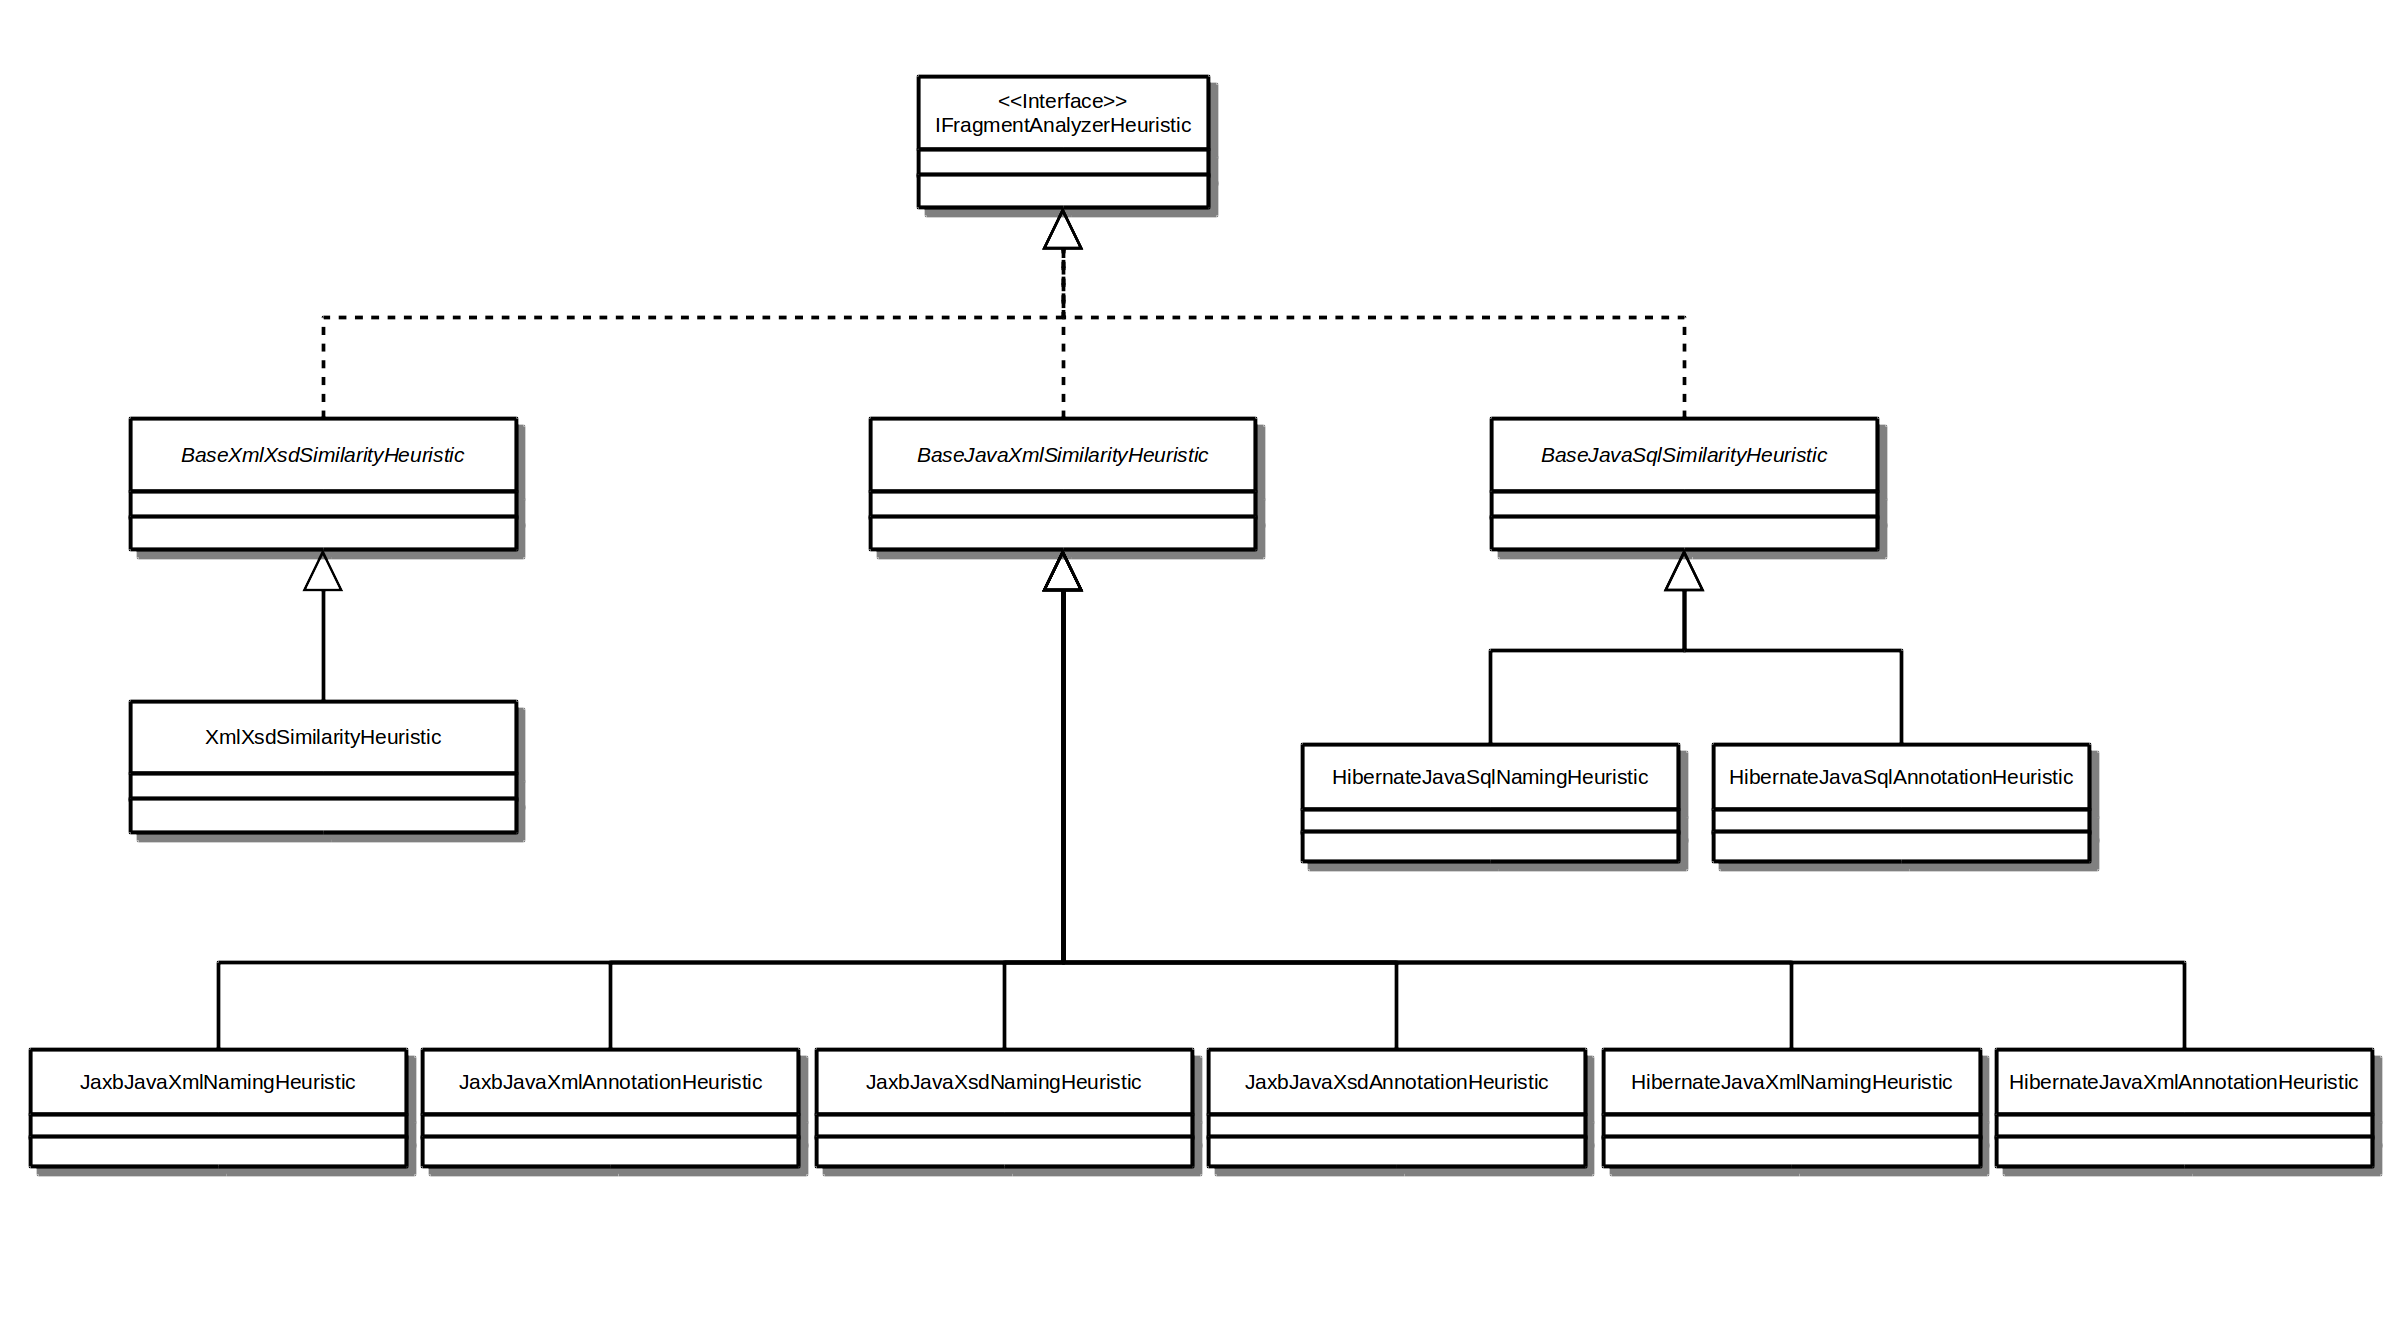
\includegraphics[width=\textwidth]{images/Heuristics.png}
\end{center}
\caption{Implemented Heuristics}
\label{figure:ImplementedHeuristics}
\end{figure}
All heuristics follow the same implementation scheme, exemplified with listings \ref{listing:ExcerptOfTheBaseXmlXsdSimilarityHeuristicClass} and \ref{listing:TheXmlXsdSimilarityHeuristicClass}.
There is an abstract base class handling traversal and concrete classes handling comparison.
Latter classes are further distinguished by the comparison tactic employed by them.
They either implement name based similarity predicates or their implementation is based on annotation meta-data.
The implemented heuristics detect:
\begin{itemize}
\item
name based similarities between \gls{XML} and \gls{XSD} \glspl{Artifact}, e.g. \gls{Conformance} links between \gls{XML} elements and \gls{XSD} complex types or \gls{Conformance} links between \gls{XML} attributes and \gls{XSD} attribute definitions;

\item
name or annotation based similarities between \gls{Java} and \gls{XML} or \gls{XSD} \glspl{Artifact} generated by \gls{JAXB}, e.g. \gls{Correspondence} links between \gls{Java} fields and \gls{XML} attributes or \gls{XSD} attribute definitions;

\item
name based similarities between \gls{Java} and \gls{Hibernate} mapping \gls{Artifact}, e.g. \gls{Correspondence} links between \gls{Java} fields and \gls{Hibernate} property mapping definitions;

\item
name or annotation based similarities between \gls{Java} and \gls{SQL/DDL} \glspl{Artifact} generated by \gls{Hibernate}, e.g. \gls{Correspondence} links between \gls{Java} fields and \gls{SQL} column definitions.
\end{itemize}